\documentclass[a4paper]{article}
\usepackage[dvips]{graphicx}
\usepackage{html} 
 \topmargin 0in
\headheight 0in
\headsep 0in
\textheight 7.7in
\textwidth 6.5in
\oddsidemargin 0in
\evensidemargin 0in
\headheight 77pt
\headsep 0.25in
\title{McStas neutron ray-trace tutorial}
\author{Peter Willendrup and Erik Knudsen, DTU Physics}
\begin{document}
\maketitle
{\noindent \small {\bf Postal adress:}\\
DTU Fysik\\Fysikvej 307\\DK-2800
  Kongens Lyngby, Denmark\\\ \\{\bf
    email:}\\\htmladdnormallink{pkwi@fysik.dtu.dk}{mailto:pkwi@fysik.dtu.dk},\htmladdnormallink{erkn@fysik.dtu.dk}{mailto:erkn@fysik.dtu.dk}}
\abstract \noindent This document is a tutorial about McStas and
neutron scattering for beginners.\\\ 
\\The text below is also included as a chapter in the McStas manual
\section{Introduction}
This tutorial has been written to help out novel users of McStas and neutron
scattering instruments. McStas is a software package for simulating
neutron scattering experiments using a Monte Carlo ray-tracing technique. This paper 
aims at helping the user to gain insight into basic neutron scattering 
as well as neutron raytracing using the McStas software package
\cite{McStas0},\cite{Manual},\cite{Websites}.
\subsection{Prerequisites}
Needed knowledge and equipment to work through the tutorial is
\begin{itemize}
\item{Undergraduate knowledge of mathematics and physics.}
\item{A computer with McStas installed (refer to the McStas
    \htmladdnormallink{homepage}{http://mcstas.risoe.dk}
    \cite{Websites} for details) or a bootable McStas Ubuntu live DVD
    (installation to harddisk possible, but not required).}
\item{This tutorial.}
\end{itemize}
\subsection{Goals and tasks}
The goals and tasks of this tutorial are
\begin{itemize}
\item{To teach you about the most basic neutron scattering.}
\item{To let you understand some of the typical components in a
    neutron scattering instrument.}
\item{To teach you basic usage of the McStas neutron simulation
    package.}
\item{To let you create your first McStas instruments, a two axis diffractometer and a triple axis spectrometer.}
\item{To teach you how to modify your instrument for a specific task.}
\item{To help you learn to debug instruments.}
\item{To help you aquire and analyze data from McStas simulations.}
\end{itemize}
\section{Basic neutron scattering}
You may recall the Bragg law from your high school physics
\[n\lambda=2d\sin(\theta),\]
giving the scattering condition for 
a wave of wavelength $\lambda$ against a series of
lattice planes with lattice spacing $d$, rotated the angle $\theta$
off the lattice plane normal. $n$ is an integer giving the spectral
order of the scattered wave. In neutron science one often refers to
the \emph{scattering vector}, $\vec{\kappa}$ of a given reflection, where
\[\kappa=|\vec{\kappa}|=n\frac{2\pi}{d}.\]
This gives us the scattering vector formulation of the Bragg law
\[\kappa=2k\sin(\theta),\]
where $k=\frac{2\pi}{\lambda}$.
%such that
%\[n\lambda=4\pi \kappa^{-1}\sin(\theta)\]
The Bragg law / scattering condition is illustrated in Figure \ref{bragg.eps}.
\begin{figure}[htb!]
\begin{center}
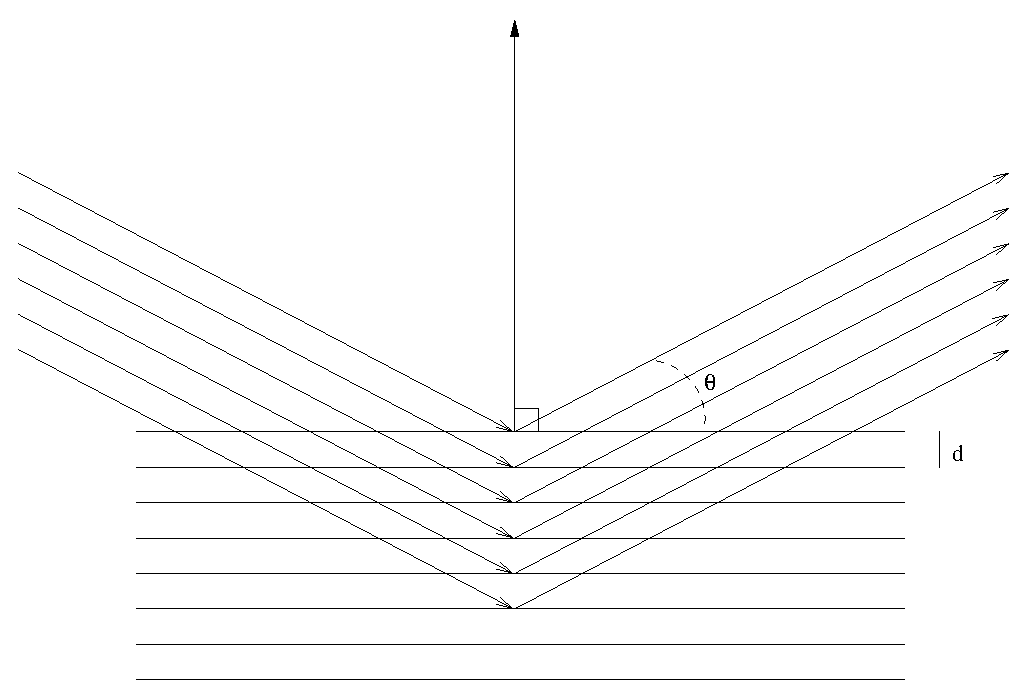
\includegraphics[width=9cm]{pics/bragg.eps}
\end{center}
\caption{Illustration of the Bragg Law.}
\label{bragg.eps}
\end{figure}
Most of the neutron processes we will study in this paper are elastic,
meaning that the wavelength of the neutron is unaltered by the process.
\section{Basic understanding of instrument components}
In the McStas formulation of a neutron scattering instrument, all
objects apart from the neutron ray are referred to as components. This
includes for instance
\begin{itemize}
\item{{\bf Source} The exit of a neutron production facility, where
    neutron rays of certain velocities are emitted into some
    portion of space.}
\item{{\bf Monochromator} (Idealized) crystal that is used to select
    neutrons of a single wavelength\footnote{In reality,
    the monochromator selects a normal distribution of wavelegths
    around $\lambda_0$, and perhaps higher orders as well ($n=2,3,...$
    in Braggs law)} $\lambda_0$ to probe the sample with (monochromator) or to 
    analyze with (analyzer).}
\item{{\bf Sample} An object altering the neutron physical properties
    in some sense, examples used here are:}
  \begin{itemize}
    \item{Vanadium. Scatters incoming neutron rays incoherently.}
    \item{PowderN. Can be thought of as a large number of crystals,
        each scattering neutron rays according to Braggs law, thereby
        producing N concentric Debye Scherrer cones. This sample also
        has the posibility of adding inchoherent, eleastically scattered
        neutron rays.}
    \end{itemize}
\item{{\bf Monitors} Objects \emph{monitoring} or registering neutron ray
    characteristics. In the exercises below are used different types
    of detectors or monitors:}
  \begin{itemize}
    \item{Monitor. Single monitor, detecting the number of neutrons flying
        through a plane. (User defined opening size).}
    \item{PSD\_monitor. Square monitor, detecting the number of
        neutron rays passing through a plane, divided into
        pixels. Square regions of a plane. (User defined resolution 
        and opening size).}
    \item{PSD\_monitor\_4PI. As PSD\_monitor but shaped like a sphere.}
    \item{L\_monitor. Wavelength monitor, measuring the different
        wavelengths of the passing neutron rays. (L is for $\lambda$).}
    \item{Monitor\_nD. General monitor for detecting all sorts of
        physical properties of the neutron ray. In our cases used with
        options:}
      \begin{itemize}
      \item{'single' - as PSD\_monitor but only one small square.}
      \item{'banana' - as PSD\_monitor but shaped like a curved,
          horizontal band.}
      \end{itemize}
    \end{itemize}
  \item{{\bf Collimators}} Devices controling the direction and divergence
   of the neutron ray.
    \begin{itemize}
      \item{Collimator\_linear} A series of parallel absorbing neutron plates
       that limits the beam divergence. 
       Typical values are $6'$ to $120'$.
    \end{itemize}
  \end{itemize}
More information on the McStas components is available by using the
\verb+mcdoc+ program (You may need to set the BROWSER system variable
to your webbrowser of choice):
\begin{itemize}
\item{\verb+mcdoc -s+ , Shows a html list of all the components}
\item{\verb+mcdoc Monitor.comp+ , Shows the documentation for a given component}
\item{\verb+mcdoc -M+ , brings up the McStas manual in PDF format}
\item{\verb+mcdoc -c+ , brings up the McStas component manual in PDF format}
\end{itemize}

\section{Basic McStas}
In short, the core of the McStas system is a precompiler. From a
user-provided instrument description, components are assembled into 
a single piece of \texttt{ansi-c} code. Using a compiler, \emph{e.g.} 
\texttt{gcc}, the c code is compiled into an executable program 
which can be run on your computer. Optionally, the program takes 
input arguments to tune the setup of your instrument/simulation. 
This section will take you through a simple example instrument 
to teach you the basic instrument language of McStas. (Instrument 
filename is vanadium\_example.instr, can be loaded using the
\verb+Neutron Site/Tutorial+ menu item of the \verb+mcgui+, see below).\vspace{1cm}
Please study \emph{carefully} the instructive comments,
marked by \verb+/* ... */+ characters
    
\begin{verbatim}
/* The line below defines the 'name' of our instrument */
/* Here, we have a single input parameter, ROT         */
DEFINE INSTRUMENT vanadium_example(ROT=0)

/* The DECLARE section allows us to declare variables  */
/* in c syntax. Here, coll_div (collimator divergence) */
/* is set to 60 arc minutes...                         */
DECLARE
%{
  double coll_div = 60;
%}

/* Here comes the TRACE section, where the actual      */
/* instrument is defined....                           */
TRACE

/* The Arm() class component defines reference points  */
/* and directions in 3D space. Every component instance*/
/* must have a unique name. Here, arm is used. This    */
/* Arm() component is set to define the origin of our  */
/* global coordinate system (AT (0,0,0) ABSOLUTE)      */
COMPONENT arm = Arm() AT (0,0,0) ABSOLUTE

/* Next, we need some neutrons. Let's place a neutron  */
/* source. Refer to documentation of Source_flat to    */
/* understand the different input parameters.          */
/* The source component is placed RELATIVE to the arm  */
/* component, meaning that modifying the position or   */
/* orientation of the arm will also affect the source  */
/* component (and other components after that one...)  */
COMPONENT source = Source_simple(radius = 0.015, dist = 1,
  xw=0.024, yh=0.015, E0=5, dE=0.2)
 AT (0,0,0) RELATIVE arm

/* Here we have a collimator - placed to improve beam  */
/* divergence. The component is placed at a distance   */
/* RELATIVE to a previous component...                 */
COMPONENT collimator = Collimator_linear(len = 0.2, 
  divergence = coll_div, xwidth = 0.04, yheight=0.06)
  AT (0, 0, 0.4) RELATIVE arm

/* We also need something to 'shoot at' - here a sample*/
/* made from vanadium - an isotrope scatterer. Options */
/* are available to restrict the solid angle in which  */
/* neutrons are emitted (no need to simulate neutrons  */
/* that we know for sure will not reach the rest of    */
/* instrument).                                        */
/* Other options for smart targeting are available -   */
/* refer to component documentation for info.          */
COMPONENT target = V_sample(thickness = 0.004, radius = 0.012, 
  yheight = 0.015, focus_r = 0, pack = 1,
  target_x = 0, target_y = 0, target_z = 1)
  AT (0,0,1) RELATIVE arm

/* Here, a secondary arm - or reference point, placed  */
/* on the sample position. The ROT parameter above     */
/* defines rotation of this arm (and components        */
/* relative to the arm)                                */
COMPONENT arm2 = Arm() 
  AT (0,0,0) RELATIVE target
  ROTATED (0,ROT,0) relative arm

/* For data output, let us place a detector. This      */
/* detector is not very realistic, since it is sphere  */
/* shaped and has a 10 m radius, but has the advantage */
/* that EVERYTHING emitted from the sample will be     */
/* picked up. Notice that this component changes       */
/* orientation with the ROT input parameter of the     */
/* instrument.                                         */
COMPONENT PSD_4pi = PSD_monitor_4PI(radius=10, nx=101, ny=51,
  filename="vanadium.psd")
  AT (0,0,0) RELATIVE arm2
END
\end{verbatim}
Enlightened by the above example, you are probably now ready to learn
a few more important details and tips about McStas.
\begin{itemize}
\item{{\bf Neutron representation:} A neutron 'history' or package is
  an entity representing a large number of neutrons. It has the
  following physical properties:
  \begin{itemize}
    \item{Spatial coordinates, $\vec{x}$ or $x,y,z$.}
    \item{Velocity components, $\vec{v}$ or $v_x,v_y,v_z$.}
    \item{Spin components, $\vec{s}$ or $s_x,s_y,s_z$.}
    \item{Time, $t$.}
    \item{Neutron weight factor, $p$.}
  \end{itemize}
\item{{\bf Neutron histories/Intensities:} McStas simulates neutron
    histories rather than direct neutron counts, \emph{i.e.} when a
    Monte Carlo choice is made in a given component (\emph{e.g.} a random
    number is generated to decide a new direction of the neutron ray), 
    the neutron \emph{weight factor} is adjusted accordingly. As you
    may have guessed already, the weight factor is the 
    average number of of observed neutrons of a given behaviour.
    The transition to direct neutron intensites is made
    by adjusting the initial neutron weight of the source component,
    so that the sum of all simulated weight factors equals the
    absolute intensity of neutrons emitted in one
    second. This means that the intensity of the neutron beam at a
    given position is the initial neutron weight multiplied by the 
    product of all the Monte Carlo weight factors occuring from the
    source to the given position.  When observing McStas output, $I$
    is the intensity, not $N$.}
\item{{\bf 3D space:} The 3D space in which the instrument is defined,
  usually has a single component which is
  placed ABSOLUTEly  in space, \emph{e.g.} at (0,0,0). All other components
  can be placed RELATIVE to this component.}
\item{{\bf Changing coordinate system:} Each component has its own
    local coordinate system. As the neutron travels from one component
    to the other, the local component coordinate system changes. The
    definition is that $z$ is the direction toward the next component,
    and that the $y$ direction is vertical. Our coordinate system is 
    right-handed, making $x$ horisontal and pointing left, looking in 
    the direction of $z$.}
\item{{\bf Component order matters!} It is important to understand
    that McStas is component order dependent. The basic idea is to
    follow the neutron as it travels from one component to the next in
    the instument description. This means that if you place one component
    \emph{geometrically} before another component, but \emph{orderly}
    after the other component, neutrons may never reach your 'first'
    component. This means that some designs can be difficult to
    achieve, though generally a solution can be found.}
\item{{\bf Use Arm()'s!} The Arm() component is very good for defining
  changed orientation of the instrument, \emph{e.g.} for axis turning points
  etc. Placing many Arm()'s will improve future flexibility of your
  instrument.}
\item{{\bf Use PSD\_monitor()'s!} The PSD\_monitor() component is a
    Position Sensitive Detector. This component can
    be used to image the shape of your beam as it travels through the
    instrument. This is very useful for debugging purposes. Other
    monitors, for instance wavelength monitors can also be useful.}}
\end{itemize}
In the McStas manual, available by clicking
\htmladdnormallink{here}{http://mcstas.risoe.dk/documentation/manual/mcstas-1.8-manual.pdf}
if you are using an internet browser to view this document, description
of usage of the different McStas tools is printed. The main McStas
programs are
\begin{itemize}
\item{\emph{mcstas} - Core application.}
\item{\emph{mcgui} - Main graphical user interface.}
\item{\emph{mcdisplay} - Ray trace / debugging application.}
\item{\emph{mcplot} - Data / display application.}
\item{\emph{mcdoc} - Documentation application.}
\end{itemize}
Here are a few hints on using the tools:
\begin{itemize}
\item To start mcgui, execute \verb+mcgui+ in a terminal window
  (\verb+mcgui.pl+ on Windows).
\item To handle instrument files (opening, editing, compiling), use \verb+File+ menu of \verb+mcgui+.
\item To simulate and plot data, use the \verb+Simulation+ menu of \verb+mcgui+.
\item To use the distributed example McStas instruments, use the \verb+Neutron Site+ menu of \verb+mcgui+.
\item For further help on usage, use the items of the \verb+mcgui+
  menu of \verb+Help+ menu or read the chapter \emph{Running McStas}
  of the McStas manual \cite{Manual}.
\end{itemize}
\section{Exercises}
Throughout the rest of this paper, you will have to do the work!
Through a series of small exercises, you will set up and use two simple
neutron scattering instruments: a diffractometer and a triple axis spectrometer. To get an idea of what your final
instrument might look like, see the sample instrument portrayed in Figure \ref{instr.eps}.

In subsection \ref{subsection:examplefile} is shown what the final exercise instrument file might look like. It is advisable to only use this file when stuck as learning by doing (yourself) is preferable to copying.
\begin{figure}[htb!]
\begin{center}
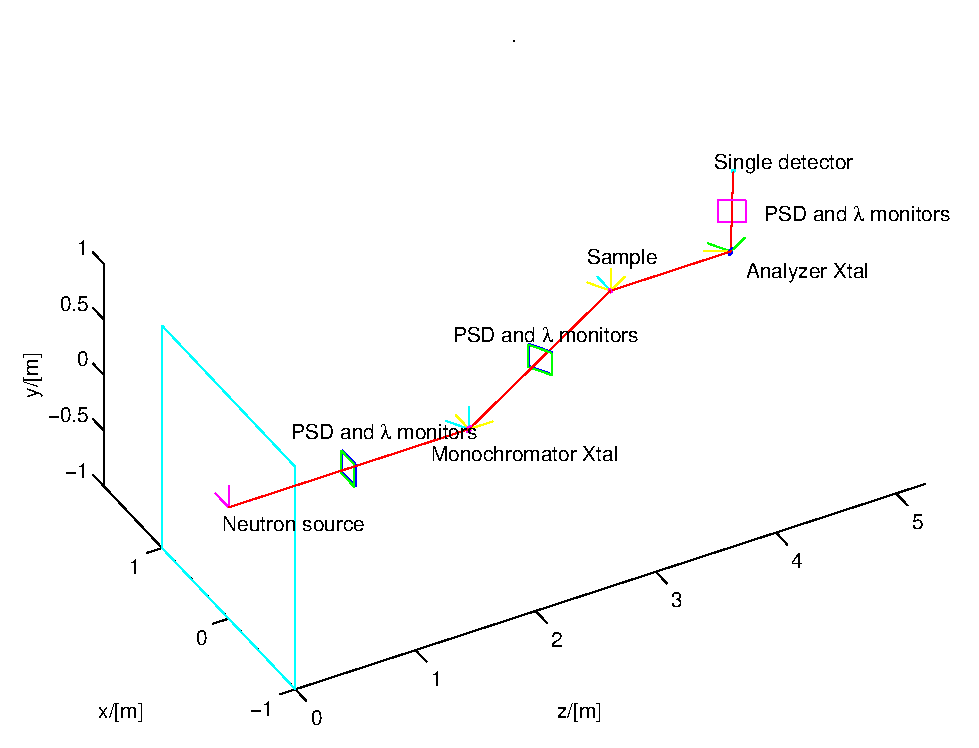
\includegraphics[width=1\linewidth]{pics/instr.eps}
\end{center}
\caption{Illustration of a triple axis diffractometer.}
\label{instr.eps}
\end{figure}
\subsection{Exercise: Source and PSD}
\begin{enumerate}
\item{Start the GUI (Graphical User Interface) by writing the command \verb+mcgui+ in a terminal. To open a terminal in Ubuntu, go to Applications $\rightarrow$ Accessories $\rightarrow$ Terminal or press Ctrl+Alt+t.}
\item{Click the Edit/New button on the GUI.}
\item{Insert a template instrument through the menu Insert $\rightarrow$ Instrument template or by pressing Alt+i twice. Set up an instrument, consisting only of an arm (keep the arm 'Progress\_bar' that is already in the file), a source (Source\_Maxwell\_3) and two monitors (a PSD\_monitor and an L\_monitor). Insert the source at (0,0,0) relative to the origin and the monitors at (0,0,1) relative to the origin. As you input each component you should read the their documentation to find the needed input parameters. The component library can be accessed by clicking the Help (McDoc) button on McGui and choosing 'Component library index'. This will open up an webpage with a list of all the components.

For the source we will help you out. Try
\begin{verbatim}
COMPONENT source = Source_Maxwell_3(
    size = 0.1, l_low = 0.1, l_high = 10, dist = 10, xw = 0.01,
    yh = 0.01, T1 = 300, T2=300, T3=300, I1=1e14, I2=0, I3=0)
AT (0, 0, 0) RELATIVE Origin
\end{verbatim}
Read the Source\_Maxwell\_3 documents using McDoc to understand the suggested parameters.}
\item{When the file is saved for the first time, McGui is automatically given the name of the instrument file. Run a simulation by pressing the Run button in McGui. After compiling the instrument file, McGui will open a window with questions on the simulation such as neutron count, \emph{i.e.} how many times a neutron ray is simulated. For now, simply press the Start button. The instrument simulation will run and its output will be given in the McGui window. When the simulation finishes, plot the results by pressing the Plot button. You should now have two plots, one from the PSD monitor and one from the wavelength monitor. If either or both of the monitors have detected no neutrons, start looking for mistakes in your instrument file.}
\item{Narrow down the interval of wavelengths emitted from the source to \emph{e.g.} l\_low=0.999 and l\_high=1.001. Rerun your simulation to check the effect. Reset the wavelength interval to [0.1 10] \AA.}
\item{Estimate the solid angle covered by your PSD. Try to understand the neutron intensity as illustrated by the plot of the registered events in the PSD in the two previous runs. Try running the simulation with half or double the number of neutron rays. Try also to vary the source focus area and to understand what you observe.}
\end{enumerate}
\subsection{Exercise: Insert a monochromator}
\begin{enumerate}
\item{Keeping your current components, insert a Monochromator\_flat component (use the component library index to get the needed parameters) and a new set of PSD and L\_monitor after the monochromator. Two new arms should be inserted to define the rotation point at the monochromator. One is used to rotate the monochromator, while the other rotates the instrument components that follow. 

Insert the two new arms at (0,0,2) relative to the origin and the monochromator at (0,0,0) relative to the monochromator arm. Also, add two new input parameters of your instrument, which we will call OMM (Omega Monochromator) and TTM (Two Theta Monochromator). These will define the angles of rotation at the monochromator as portrayed in Figure \ref{mono.eps}. 
\begin{figure}[htb!]
\begin{center}
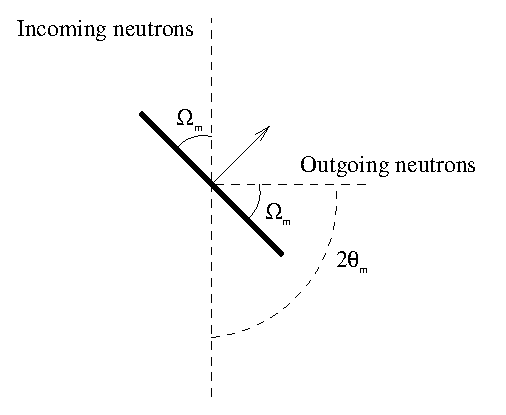
\includegraphics[width=8cm]{pics/mono.eps}
\end{center}
\caption{Illustration of the monochromator orientation.}
\label{mono.eps}
\end{figure}}
\item{Given $\lambda$ = 4\AA, and knowing that for the monochromator $\kappa=1.8734$ \AA$^{-1}$ (Pyrolytic Graphite), use Bragg's law to determine the correct Bragg angle (\emph{i.e.} OMM/TTM) of the monochromator for the $n=1$ reflection. Add the OMM and TTM input parameters to the DEFINE line at the beginning of the instrument file and give them the values you just calculated. Rotate the two arm components by OMM and TTM.}
\item{Do a scan of OMM a couple of angles around the determined Bragg value to verify the finding, while keeping TTM fixed. This is done by replacing the fixed value of OMM in the Run Simulation window with two numbers separated by a comma, \emph{e.g.} 20,25. These numbers represent the minimum and maximum values of OMM. A number of steps must also be given and this is done by changing the \# steps value from 1 to \emph{e.g.} 10. Check the position of the peak on the PSD and the wavelength on the L\_monitor. }
\item{What should $\kappa$ be set to to get the $n=2$ reflection at exactly OMM$=45^\circ$ (TTM$=90^\circ$)? Adjust $\kappa$ for the monochromator and verify the calculation by a scan. Check the wavelength by plotting the scan.}
\item{Determine the Bragg angle for the $n=1$ reflection in this setting of $\kappa$ and verify it by scanning OMM. Set OMM to this value. Perform the simulation and check the wavelength distribution. Comment.}
\item{Before you go on, change the minimum and maximum wavelengths of the source to a suitably narrow interval around 4\AA. There is no need to produce neutron rays that will not be scattered at the monochromator.}
\end{enumerate}
\subsection{Exercise: Insert a sample}
\begin{enumerate}
\item{Now, insert a \verb+V_sample()+ component after the last PSD\_monitor and L\_monitor and a Beamstop component 1.5 m after the sample. The \verb+V_sample()+ component simulates a Vanadium sample. Such a sample scatters incoherently, \emph{i.e.} in all directions. At the same position as the sample, insert a PSD\_monitor\_4PI component of radius 1.0 m. Read the documentation for details on input parameters. Run a simulation. Notice the number of hits.}
\end{enumerate}
\subsection{Exercise: Insert a sample with two powder lines}
\begin{enumerate}
\item{Next, let us insert something more interesting. Remove the V\_sample and  PSD\_monitor\_4PI and insert a PowderN component with the following parameters:
    \begin{verbatim}
COMPONENT sample = PowderN(radius=0.01,h=0.01, d_phi0=0.1, pack=0.5, 
   DW=0.9, frac=0.5, reflections="mylist.dat",
   Vc=3.86*3.86*11.82, sigma_abs=0, sigma_inc=2, barns=1)
  AT (0, 0, 0) RELATIVE \<name of arm at the sample position\>
\end{verbatim}
You should also create a list of reflections and save it as \texttt{mylist.dat}. The list should have the following contents:
\begin{verbatim}
# column_j 3 multiplicity 'j'
# column_q 1  Scattering vector modulus [Angs^-1]
# column_F2 2 Scattering factor |F^2| in [barns]
1 10 8
1.3 10 4
\end{verbatim}
}
\item{Insert a banana shaped detector:
\begin{verbatim}
COMPONENT BananaDetector = Monitor_nD(
   xwidth=2, yheight = 0.09, 
   options="banana, theta limits [-55 -35] bins=360, file =detector.dat")
  AT (0,0,0) RELATIVE sample
\end{verbatim}
and make sure that the previously inserted beamstop is after the banana detector in the component list. Test that neutrons reach the detector by running a simulation. 

Afterwards, choose trace instead of simulate in the Run simulation window and see the instrument, you have created. To see only the trace of the neutrons, which hit the detector, select the detector component in the list given in the Inspect component box. Also, insert the following after the sample component:
\begin{verbatim}
EXTEND %{ 
if (!SCATTERED) ABSORB;
%}
\end{verbatim}
This will insert a command in c-language into the compiled instrument file. The command says that if the simulated neutron does not scatter at the sample, it is absorbed. This removes the direct beam and should be used with caution.}
\end{enumerate}
\subsection{Exercise: Insert a real sample}
\begin{enumerate}
\item{Instead of \texttt{mylist.dat} use \texttt{Na2Ca3Al2F14.laz}. Change the limits of the banana detector to [-10 -130] and change the sample component to read:
\begin{verbatim}
COMPONENT sample = PowderN(
    reflections = "Na2Ca3Al2F14.laz", d_phi = 0.1, radius = 0.004,
    h = 0.03, DW = 0.9, barns = 1, pack = 0.7, frac = 0, tfrac=0)
  AT (0, 0, 2) RELATIVE arm2
\end{verbatim}

Make a simulation to check that a nice powder pattern is observed. If it is time for a coffee break, close the plot from the quick run and instead do a long simulation, \emph{e.g.} 20 million neutron rays, and have coffee.}
\end{enumerate}
\subsection{Exercise: Insert an analyzer}
\begin{enumerate}
\item{Comment out the banana detector and beamstop with /* and */ before and after the components, respectively. Copy the banana detector, but make it to a single detector by changing the options for the Monitor\_nD component to ``single''.}

\item{Add an arm at the sample and an angle to rotate the part of the instrument located after the sample, \emph{e.g.} TT (Two $\Theta$) and decide a more relevant size of the now rectangular detector. Look at your results from the last simulation to determine an approximate scan range for the TT angle, \emph{e.g.} -66.5,-67.5, which will make a scan around the peak at $2\theta=66.94^{\circ}$. Scan TT across one or more powder lines.}

\item{Between sample and detector, set up an analyser crystal by copying and modifying your monochromator component. Add new arms and angles: OMA and TTA; A is for Analyzer. Adjust the analyser to Bragg condition for the chosen wavelength. Re-scan TT and notice the difference to the scan performed in the previous task. Try also scanning around -TT and notice the difference to the other scan. Can you explain the difference?}
\end{enumerate}
\subsection{Example instrument file}\label{subsection:examplefile}
\begin{verbatim}
/*******************************************************************************
*         McStas instrument definition URL=http://www.mcstas.org
*
* Instrument: test (rename also the example and DEFINE lines below)
*
* %Identification
* Written by: Your name (email)
* Date: Current Date
* Origin: Your institution
* Release: McStas CVS-080208
* Version: 0.2
* %INSTRUMENT_SITE: Institution_name_as_a_single word
*
* Instrument short description
*
* %Description
* Instrument longer description (type, elements, usage...)
*
* Example: mcrun test.instr <parameters=values>
*
* %Parameters
* Par1: [unit] Parameter1 description
*
* %Link
* A reference/HTML link for more information
*
* %End
*******************************************************************************/

/* Change name of instrument and input parameters with default values */
DEFINE INSTRUMENT test(OMM=36.607, TTM=73.214, TT=-66.94, OMA=36.607, TTA=73.214)

/* The DECLARE section allows us to declare variables or  small      */
/* functions in C syntax. These may be used in the whole instrument. */
DECLARE
%{
%}

/* The INITIALIZE section is executed when the simulation starts     */
/* (C code). You may use them as component parameter values.         */
INITIALIZE
%{
%}

/* Here comes the TRACE section, where the actual      */
/* instrument is defined as a sequence of components.  */
TRACE

/* The Arm() class component defines reference points and orientations  */
/* in 3D space. Every component instance must have a unique name. Here, */
/* Origin is used. This Arm() component is set to define the origin of  */
/* our global coordinate system (AT (0,0,0) ABSOLUTE). It may be used   */
/* for further RELATIVE reference, Other useful keywords are : ROTATED  */
/* EXTEND GROUP PREVIOUS. Also think about adding a neutron source !    */
/* Progress_bar is an Arm displaying simulation progress.               */
COMPONENT Origin = Progress_bar()
  AT (0,0,0) ABSOLUTE

COMPONENT Source_Maxwell_3 = Source_Maxwell_3(
    size = 0.05, l_low = 3.9, l_high = 4.1, dist = 10, xw = 0.01,
    yh = 0.01, T1 = 150.42, T2 = 38.74, T3 = 14.84, I1 = 3.67E11, I2 = 3.64E11,
    I3 = 0.95E11)
  AT (0, 0, 0) RELATIVE Origin

COMPONENT L_monitor = L_monitor(
    filename = "test2.psd", xmin = -0.1, xmax = 0.1, ymin = -0.1,
    ymax = 0.1, Lmin = 2.1, Lmax = 6)
  AT (0, 0, 1) RELATIVE Origin

COMPONENT PSD_monitor = PSD_monitor(
    nx = 90, ny = 90, filename = "test.psd", xmin = -0.1,
    xmax = 0.1, ymin = -0.1, ymax = 0.1)
  AT (0, 0, 1) RELATIVE Origin

COMPONENT arm1 = Arm()
  AT (0, 0, 2) RELATIVE Origin
  ROTATED (0, OMM, 0) RELATIVE Origin

SPLIT 10 COMPONENT Monochromator_flat = Monochromator_flat(
    zmin = -0.1, zmax = 0.1, ymin = -0.1, ymax = 0.1,
    mosaich = 30, mosaicv = 30)
  AT (0, 0, 0) RELATIVE arm1
EXTEND %{ 
if (!SCATTERED) ABSORB;
%}

COMPONENT arm2 = Arm()
  AT (0, 0, 2) RELATIVE Origin
  ROTATED (0, TTM, 0) RELATIVE Origin

COMPONENT L_monitor2 = L_monitor(
    filename = "test3.psd", xmin = -0.1, xmax = 0.1, ymin = -0.1,
    ymax = 0.1, Lmin = 2.1, Lmax = 6)
  AT (0, 0, 1) RELATIVE arm2

COMPONENT PSD_monitor2 = PSD_monitor(
    nx = 90, ny = 90, filename = "test4.psd", xmin = -0.1,
    xmax = 0.1, ymin = -0.1, ymax = 0.1)
  AT (0, 0, 1.01) RELATIVE arm2

SPLIT 10 
COMPONENT sample = PowderN(
    reflections = "Na2Ca3Al2F14.laz", d_phi = 0.1, radius = 0.004,
    h = 0.03, DW = 0.9, barns = 1, pack = 0.7, frac = 0, tfrac=0)
  AT (0, 0, 2) RELATIVE arm2

/*COMPONENT sample = PowderN(
    reflections = "mylist.dat", d_phi = 0.1, radius = 0.01,
    Vc = 3.86*3.86*11.82, sigma_abs = 0, sigma_inc = 2, h = 0.01,
    DW = 0.9, barns = 1, pack = 0.5, frac = 0.5)
  AT (0, 0, 2) RELATIVE arm2*/
EXTEND %{ 
if (!SCATTERED) ABSORB;
%}

COMPONENT arm3 = Arm()
  AT (0, 0, 0) RELATIVE sample
  ROTATED (0, TT, 0) RELATIVE sample

/*COMPONENT BananaDetector = Monitor_nD(
    xwidth = 2, yheight=0.09, 
    options="banana, theta limits [-10 -130] bins=360, file =detector.dat")
  AT (0, 0, 0) RELATIVE sample

COMPONENT STOP2 = Beamstop(radius=0.3)
AT (0,0,3.5) RELATIVE arm2*/

COMPONENT PSD_monitor3 = PSD_monitor(
    nx = 90, ny = 90, filename = "test5.psd", xmin = -0.132,
    xmax = 0.132, ymin = -0.02, ymax = 0.02)
  AT (0, 0, 0.5) RELATIVE arm3

COMPONENT arm4 = Arm()
  AT (0, 0, 1) RELATIVE arm3
  ROTATED (0, OMA, 0) RELATIVE arm3

SPLIT 10 COMPONENT AnalyzerCrystal = Monochromator_flat(
    zmin = -0.1, zmax = 0.1, ymin = -0.1, ymax = 0.1,
    mosaich = 30, mosaicv = 30)
  AT (0, 0, 0) RELATIVE arm4

COMPONENT arm5 = Arm()
  AT (0, 0, 0) RELATIVE AnalyzerCrystal
  ROTATED (0, TTA, 0) RELATIVE arm3

COMPONENT Analyzer = Monitor_nD(
    xwidth = 0.01, yheight=0.1, 
    options="single, file = analyzer.dat")
  AT (0, 0, 1) RELATIVE arm5



/* This section is executed when the simulation ends (C code). Other    */
/* optional sections are : SAVE                                         */
FINALLY
%{
%}
/* The END token marks the instrument definition end */
END
\end{verbatim}
\section{Suffix}
Well done, you have come to the end of the McStas tutorial. Hopefully,
most of the goals of the tutorials have been fulfilled. Otherwise,
feel free to contact the
\htmladdnormallink{authors}{mailto:peter.willendrup@risoe.dk,kim.lefmann@risoe.dk}
of this paper or the \htmladdnormallink{McStas users
  mailinglist}{mailto:mcstas-users@mcstas.org} for further help.

\begin{thebibliography}{10}
\bibitem{McStas0}
K. Lefmann and K. Nielsen: \emph{McStas, a general software package
  for neutron ray-tracing simulations}, Neutron News, {\bf 10} pp. 20-23, 1999

\bibitem{Manual}
P. Willendrup, E. Farhi K. Lefmann et. al.: \emph{User and Programmers
  Guide to the Neutron Ray-Tracing Package McStas, Version 1.11}, Ris\o\
National Laboratory, Roskilde, Denmark, January 2007\\
\bibitem{Component Manual}
P. Willendrup, E. Farhi K. Lefmann et. al.: \emph{Component Manual for
 the Neutron Ray-Tracing Package McStas, Version 1.11}, Ris\o\
National Laboratory, Roskilde, Denmark, January 2007\\

\bibitem{Websites}
McStas homepage: \url{http://www.mcstas.org}\\
\end{thebibliography}



\end{document}